%%%%%%%%%%%%%%%%%%%%%%%%%%%%%%%%%%%%%%%%%%%%%%%%%%%%%%%%%%%%%%%%%%%%%%%%
% Template for a Master's Thesis or Ph.D. dissertation
% at the University of Wisconsin-Milwaukee.
%
% Designed for LaTeX version 2e
%
% Updated by Adam J. Smith
% December, 2007
%
% This thesis template requires the file "UWMthesis.sty", available
% on the UWM's Atmospheric Science Club website, and possible in other
% locations.
%
% A LaTeX primer is not provided here.  For instructions on how to use commands for
% figures, table, equations, and bibliography citations, please see the documentation
% listed later in this document.
% 
% This template follows the "Fall 2007" version of the 
% University of Wisconsin-Milwaukee standards for the Master's thesis
% and Ph.D. dissertation.  Please feel free to update this template
% as needed to comply with these standards.
%
% For current thesis and dissertation formatting information, visit the UWM graduate school
% website at the following address:
% http://www.graduateschool.uwm.edu/students/current/thesis-and-dissertation-formatting/
%
% IMPORTANT: Be sure to meet with the appropriate Graduate School personnel to verify
% whether your final document meets the UWM standards.  If not, the document may not
% be accepted until any problems are corrected.
%%%%%%%%%%%%%%%%%%%%%%%%%%%%%%%%%%%%%%%%%%%%%%%%%%%%%%%%%%%%%%%%%%%%%%%%

% If you are writing a master's thesis, use the first option (master).
% If you are writing a phd dissertation, use the second option (phd).
\documentclass[master]{UWMThesis}
%\documentclass[phd]{UWMThesis}

%------------------------------------

% Uncomment the following "usepackage" line if you wish to use BiBTeX to create the
% bibliography.  This package is necessary to use the \citep or \citet commands, which are
% commonly used in publications like the Journal of Geophysical Research.
% If the style file "natbib.sty" is not provided with your release of MiKTeX, it is available
% on the Internet.  One example web source is:
% http://ads.harvard.edu/pubs/bibtex/astronat/natbib.sty
\usepackage{natbib}

%------------------------------------

% Uncomment this package if you want to use graphics files, such as .eps files
\usepackage{graphicx}

% Other packages go here as needed...
%\usepackage{mathabx}
\usepackage{showframe}
%------------------------------------

% Insert your full name in the brackets.
\renewcommand{\ThesisAuthor}{First M. Last}

% If you are graduating in Spring, insert May.  If you are graduating in Fall, insert December.
\renewcommand{\ThesisMonth}{May}

% Insert the year of your graduation here
\renewcommand{\ThesisYear}{2008}

% Your thesis title goes here.  It will automatically be formatted to use multiple lines
% (if needed)
\renewcommand{\ThesisTitle}{Your thesis title: An analysis of the correlation between long thesis titles and the amount of interest expressed by the scientific community}

% Insert your advising professor's name here.  DO NOT include a prefix of "Prof." or "Dr."
% here!  The prefix will be inserted automatically.
\renewcommand{\ThesisAdvisor}{Genius B. Advisor}

%------------------------------------

% If your thesis or dissertation has multiple volumes, set the argument to true.
% If not, set the argument to false.
\setboolean{multvolumes}{false}

% If your thesis or dissertation has multiple appendices, set the argument to true.
% If not, set the argument to false.
\setboolean{singleappendix}{false}

%---------------------------------------

% Creating new commands for displaying derivatives
% Add additional new commands as needed...
\newcommand{\ptlder}[2]{\frac{\partial #1}{\partial #2}}
\newcommand{\totder}[2]{\frac{d #1}{d #2}}

%---------------------------------------

% BEGINNING OF DOCUMENT
\begin{document}

% Formatting initial pages 
\ThesisFrontmatter

%---------------------------------------

% Creating the title page and approval page.  This is done automatically using commands
% in UWMThesis.cls.
\ThesisTitlepage

%---------------------------------------

% Begin typing the abstract here.  The thesis title and author will be included on this page.
\begin{ThesisAbstract}
Summarize your paper here, including the basic methods used in the study.
A signature line for your advisor will be included at the end of the abstract.

NOTE: The abstract can have multiple pages, but is restricted to 400 words in length!
\end{ThesisAbstract}

%--------------------------------------

% If you want a copyright page, uncomment these lines.  The text will be inserted automatically.
\newpage
\ThesisCopyright

%--------------------------------------

% If you want a dedication page, uncomment this line
\ThesisDedication{To Dr. Rossby} % optional

%--------------------------------------

% The next few sections must be single-spaced
\begin{singlespacing}

% Adding table of contents (REQUIRED!)
% The entries are created automatically, based on your use of "\chapter" and "\section".
\tableofcontents

% Adding a list of figures (REQUIRED IF YOU USE FIGURES!)
% Each entry is created automatically when you add
% a "\figure" command.
% If you don't have figures in your thesis, comment this line out.
\listoffigures	%only if figures in text

% Adding a list of tables (REQUIRED IF YOU USE TABLES!)
% Each entry is created automatically when you add
% a "\table" command.
% If you don't have tables in your thesis, comment this line out.
\listoftables	% only if tables in text

%--------------------------------------

% A list of symbols is only required if you don't describe variables within the text.
% Consult with your advisor to find the best way to list your symbols.  It may also be useful
% to use a glossary package (e.g. nomencl.sty).  

% If you need to use a list of symbols, insert them here.
% Otherwise, comment this section out.

% Place the symbol on the left, then an \hfill command, then the variable description.
% (The \hfill command places the variable description at the right side of the page, with
%  white space separating the two entries.)

\begin{center}{\clearpage\textbf{\Large \sc List of Symbols}}\end{center} %\vspace*{8ex}

$\Gamma$ \hfill Dry adiabatic lapse rate \vfill\clearpage

\end{singlespacing}

%--------------------------------------

% Insert acknowledgements here.  Be sure to include those who have provided important
% information for your project.  It is also customary to thank others who have assisted
% in your research, or include personal thank-yous.

% DON'T FORGET TO ADD ANY COPYRIGHTS THAT MAY BE REQUIRED!  If you don't, the Library may not
% approve your thesis.

\begin{ThesisAcknowledgement}
Here is a section for acknowledgements.  Be sure to thank your advisor...

First, I would like to thank Dr. Vincent E. Larson for advising me on this project....

Also, be sure to thank your key collaborators, including those that provided information or assistance...

I also need to thank those who have provided me with critical information during this study, including Dr. Larry Carey (ESSC / University of Alabama Huntsville) and Dr. Jianguo Niu (Texas A\&M University) for providing aircraft observations, and Dr. J. Adam Kankiewicz for providing LBF rawinsonde data.  Dr. Jean-Christophe Golaz (NOAA / GFDL) has been invaluable in providing developmental assistance with the COAMPS-LES model.

You may also wish to include a few personal acknowledgements.  Be brief but thorough.

Finally, include any necessary copyrights...

COPYRIGHT NOTICE: COAMPS\textregistered is a registered trademark of the Naval Research Laboratory.

{\textit{
Document note: This thesis template was originally provided by Dr. Richard Stockbridge of the UWM Math Department, Fall 2007.  It was updated by Adam J. Smith in January 2008.  All related files may be modified as needed to conform with current UWM thesis rules and requirements.
}}
\end{ThesisAcknowledgement}

%------------------------------------

% If you want to include a quote or some intersting tidbit, insert it here.
% Otherwise, comment it out.
\ThesisFrontispiece{\begin{singlespacing}If you wish, add an optional quote or tidbit: \\
I spent a lot of money on booze, birds and fast cars. The rest I just squandered.\end{singlespacing}\\ \hfill{\itshape{George Best}}}	%optional

%------------------------------------

% Reformatting page style for the main body
\ThesisMainmatter

%------------------------------------
%------------------------------------

% To start a new chapter in the document, use the "\chapter" command.
% The heading is defined by the argument.
% (An entry will be automatically added to the table of contents for each new chapter.)
\chapter{Introduction} \label{sec:intro}

Begin with an introduction, which describes the reason for your research.  Begin with a broad focus, and then being focusing more on your topic.  At the end, introduce your specific project, and provide general information on what your thesis will cover.  Leave the details for the other sections of the thesis.

Throughout this document, feel free to replace any text, figures, tables, labels, etc. with your own material.  Chapters and sections may be replaced, renamed or omitted as needed.

Be sure to retain all commands such as \verb=\begin{ThesisAbstract}=.  These commands are required in order to produce the right document formatting.  If you are in doubt, leave the command alone, or see the example thesis document provided along with this template.

EXAMPLE INTRODUCTION, WITH CITATIONS:

Midlevel ``alto" clouds, such as altostratus or altostratocumulus \citep{larson_et_al_06a}, are thin clouds, typically less than 1000m thick.  The clouds are generally overcast, meaning that they have cloud fractions of nearly one.  In addition, alto clouds may contain both liquid and ice particles, meaning they could be ``mixed-phase".  They can occur in any climate region \citep{sassen_khvorostyanov_07a}, and they cover up to 22\% of the planet's surface at any given time \citep{warren_et_al_88a,warren_et_al_88b}.

Continue with the rest of your introduction here...

%-----

% To add another chapter, use another "\chapter" command.
\chapter{Next chapter: figures}  \label{sec:chap_figs}

Here, we begin our next chapter using the \verb=\chapter= command.  Use chapters to separate the different parts of your thesis.

In an actual thesis, the second chapter would probably describe methodology.  However, in this document we will provide explanations on the LaTeX commands you will probably need.

First, we discuss how to generate figures.  To do so, we create a new section, using the \verb=\section= command.  Sections are great for dividing up specific pieces within a chapter.

	% For divisions within a chapter, use the "\section" command.
	% A new table of contents entry will be placed underneath the chapter heading.
	\section{Figures 1} \label{sec:fig1}
  In LaTeX, all figures need to be in a PostScript type format, such as EPS.  This format allos for easy resizing without distorting the original image.  EPS documents can be created in Matlab or through other programs such as Adobe Photoshop.
	
	Here we create a figure (using the \verb=\begin{figure}= command).  The syntax for the figure is as follows:

\begin{verbatim}
\begin{figure}[h]
 \centering
 \noindent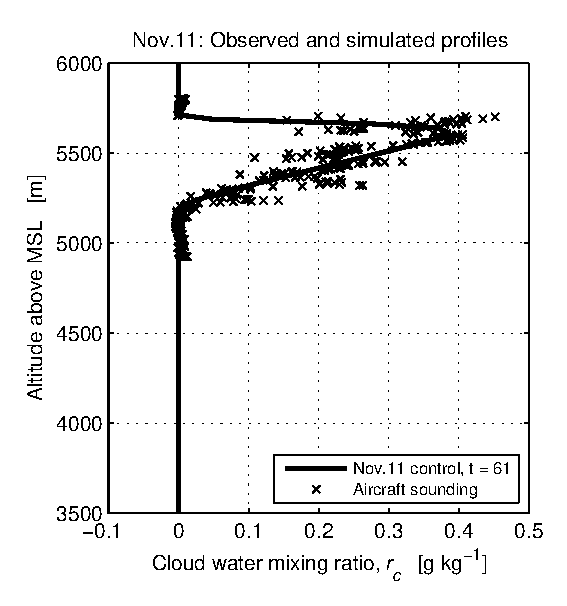
\includegraphics[width=20pc]
    {./nov11_sndg_qcm_compare_t61_bw.eps}
 \caption{A comparison of simulated liquid water mixing ratio
          ($r_c$) in the Nov.11 control simulation versus the
          available aircraft sounding....}
 \label{fig:nov11_init_qcm}
\end{figure}
\end{verbatim}

By using the above syntax, we produce the following figure:

\begin{figure}[h]
 \centering
 \noindent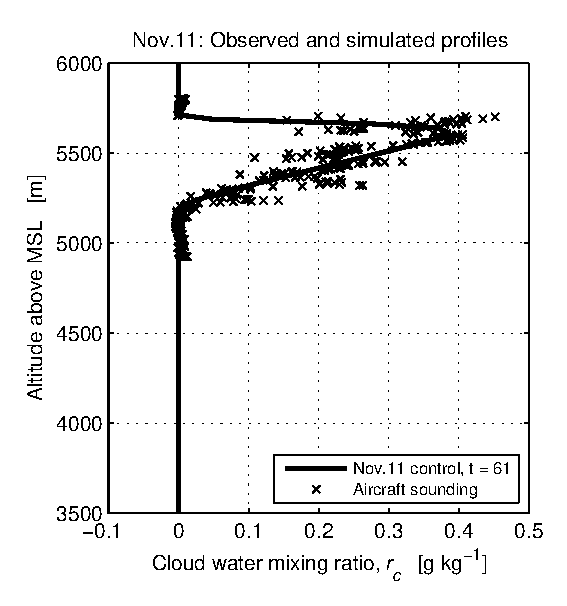
\includegraphics[width=20pc]
    {nov11_sndg_qcm_compare_t61_bw.eps}
 \caption{An example caption: A comparison of simulated liquid water mixing ratio
          ($r_c$) in the Nov.11 control simulation versus the
          available aircraft sounding.}
 \label{fig:nov11_init_qcm}
\end{figure}

A few notes on the syntax:

The \verb=[h]= option denotes that the figure should be placed ``here" in the document, at the specified location between specific paragraphs of text.  However, if the figure is too big to place ``here", LaTeX will automatically switch to the [ht] option, which places the figure at the top of the next page.  If this occurs, a warning will be displayed during rebuilding.

The \verb=[width]= option denotes the width of the figure, in a unit called ``picos".  Adjusting the number will resize the figure to the new setting.  Figures are automatically resized equally in both the horizontal and vertical to prevent distortion.

After the \verb=[width]= option, we include the filepath to the desired graphic file.  The filename must be placed in curly brackets.  Here, the graphics file is in the same directory as the TeX file, so we only need to include the filename.  However, you can also include files from other directories, using a full filepath (as in \verb=/home/ajsmith4/thesis_figures/graphic.eps=) or a relative filepath (as in \verb=../thesis_figures/graphic.eps=).

Next is the \verb=\caption= command.  This command generates the caption for the figure.  All parts of the caption must be within the curly brackets.  Feel free to use any text, variables or references (\verb=\ref= commmand) as needed.  Include an explanation the main figure information, such as what each line or symbol stands for.  Do not use the caption to describe the meaning behind the figure, but instead leave that information for the main text.  Keep in mind that the caption will be listed in the Table of Figures that is generated at the beginning of your thesis.

Finally, you can use a \verb=\label= to identify your figure within the thesis document.  Labeling is discussed later.

Be sure to end the figure section with \verb=\end{figure}=.  Otherwise, errors will occur.

%-----

For a UWM thesis or dissertation, it may be better to place all figures together.  If you choose this option, all figures must appear at the end of the relevant chapter.  You can still use the same syntax as before.

We will display one more figure at the end of this chapter, to show the second method of displyaing figures.  Note that this second figure is given a width of 35pc (picos), so the figure will be sized bigger.  In fact, it is too big to fit on this page, so it is moved to the next page (with a LaTeX warning during rebuilding). Also note that this figure is in color.  Color is acceptable in your final submission, as long as all of your symbols or lines are distinguishable.

\begin{figure}[ht]
 \centering
 \noindent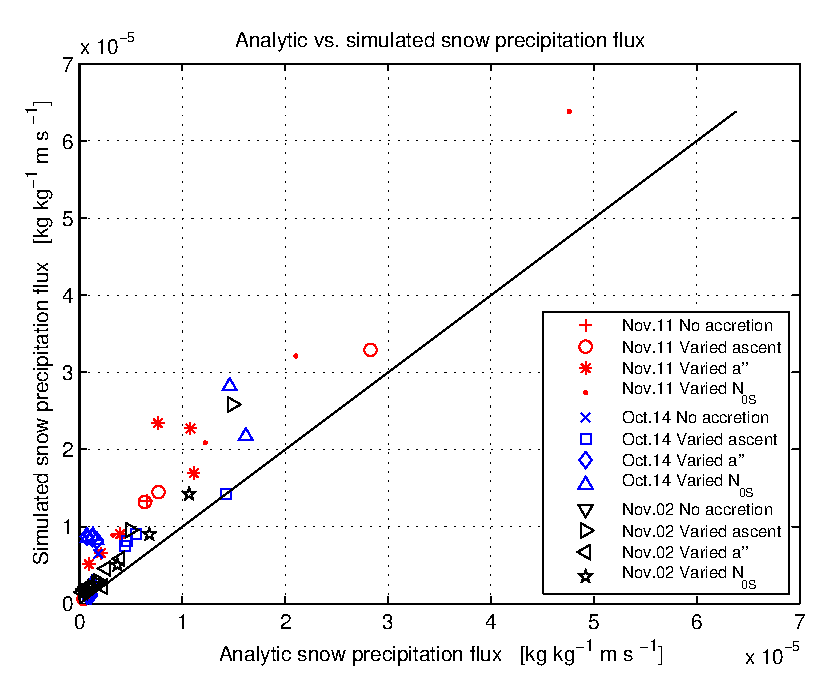
\includegraphics[width=35pc]{scatter_eqn23_F_psdep.eps}
 \caption{A second figure at the end of the chapter: Comparing calculated snow precipitation flux from a diagnostic equation (x-axis) versus simulated snow precipitation flux (y-axis).} 
                             \label{fig:scatter_F_psdep}
\end{figure}

%------------------------------------

\chapter{Creating symbols and equations}  \label{sec:equations}

It can be very useful to create symbols or equations in your document.  To create variables or equations within the text, we use a pair of dollar signs (\$\$).  Anything within the dollar signs will be translated in ``math mode", which allows the user to generate equations, subscripts, exponents, fractions, etc.

For example, we can use different syntax to do the following:

\begin{center}
For a fraction, \verb=$\frac{x}{2}$= yields $\frac{x}{2}$

For an exponent or superscript, \verb=$x^2$= yields $x^2$

For a subscript, \verb=$r_c$= yields $r_c$

For a simple equation, \verb|$x+1=3$| yields $x+1=3$.
\end{center}

LaTeX also has many symbols and other options.  The program TeXnicCenter provides many commands for symbols or formatting options.  Just look in the toolbar and menus.  For more information on specific formatting or symbols, consult a LaTeX documentation (see the end of this document).

\section{A single-line equation}  \label{sec:single_line_eq}.

Most equations must be emphasized and numbered.  To do so, use the \verb=equation= environment as follows:

\pagebreak

\begin{verbatim}
\begin{equation}
    \ptlder{r_S}{t} = - \ptlder{(\overline{w_S} r_S)}{z}
                      + \frac{\mathrm{PSDEP}}{\rho}.
    \label{eq:snow_budget}
\end{equation}
\end{verbatim}

This syntax produces the following output:

\begin{equation}
    \ptlder{r_S}{t} = - \ptlder{(\overline{w_S} r_S)}{z}  + \frac{\mathrm{PSDEP}}{\rho}.
    \label{eq:snow_budget}
\end{equation}

NOTE: The command \verb=\mathrm= removes the italics from the specified text.  Thus, the variable (e.g. PSDEP) will actually appear to have normal text.

When using the equation environment, we do not need to include dollar signs, since math mode is automatically presumed.  Equation numbering is produced automatically, based on the current chapter number and the order of equations in the chapter.  We also use a \verb=\label= command, which is discussed later.

In the \verb=equation= environment, the equation will be displayed on a single line, regardless of the length.  If the equation is too long, it will overlap the page margins and may even be cut off by the page boundaries.  Therefore, it may be necessary to use another display option.

%-----

\section{A multi-line equation} \label{sec:multi_line_eq}

Many equations are too long to be displayed on a single line.  However, the command \verb=\eqnarray= can be used to display equations on multiple lines.  Here is an example of an equation that uses the \verb=\eqnarray= command:

\pagebreak

\begin{verbatim}
\begin{eqnarray}
	\left< \ptlder{r_c}{t} \right> 
	    & = & \mathrm{Mix}_{r_c}
	          + \mathrm{Ascent}_{r_c} + \mathrm{Rad}_{r_c} \nonumber \\
	    & + & \mathrm{PSACW}_{r_c} + \mathrm{PSDEP}_{r_c}
	          + \mathrm{PDEPI}_{r_c},
	\label{eq:liq_budget_equation}
\end{eqnarray}
\end{verbatim}

This syntax will produce the following equation:
\begin{eqnarray}
	\left< \ptlder{r_c}{t} \right> & = & \mathrm{Mix}_{r_c} + \mathrm{Ascent}_{r_c} + \mathrm{Rad}_{r_c} \nonumber \\
	                               & + & \mathrm{PSACW}_{r_c} + \mathrm{PSDEP}_{r_c} + \mathrm{PDEPI}_{r_c},
	\label{eq:liq_budget_equation}
\end{eqnarray}

A few details to note:

\begin{enumerate}
\item The \& symbol is used to define how LaTeX should align the different lines.  In the example equation, the \& symbols are used to align the equal sign (=) and the plus sign (+).

\item Use a double backslash (\verb=\\=) to end each line.

\item The \verb=eqnarray= environment can also be used to display multiple steps, such as when describing a derivation.

\item In this environment, each row will be numbered unless you include the command  \verb=\nonumber= in that row.

\item Be sure to rebuild the code and check the resulting output often.  Make sure the equation looks good, and that it does not create a ``bad box" by crossing the page margins.

\end{enumerate}

Of course, there are other methods for creating equations, which are detailed in LaTeX documentations.  Please consult those sources if you are interested.

%------------------------------------

\chapter{Adding data tables} \label{sec:data_tables}
Sometimes it may be useful to add data in a table.  Here, the syntax is much more complicated, and is not included in the PDF output.  To view the actual syntax, please see the TeX file.

We can use the following table to describe simulation settings:

\begin{table}[h]
\centering
\caption{Imposed sensitivity values of large-scale vertical velocity ($V_{ls}$) for simulated COAMPS-LES cloud cases.  Positive values indicate ascent.  In each sensitivity study, a single value of ascent or descent is selected.  All other parameters are set to their control values.  An asterisk denotes the control setting for each cloud case.}
\vspace{0.5pc}
\begin{tabular}{c|cccccc}
\hline
Cloud case & \multicolumn{5}{c}{Imposed vertical velocity settings} \\
\hline
Nov.11 & -5 cm s$^{-1}$ & -3 cm s$^{-1}$* & -1 cm s$^{-1}$ &   1 cm s$^{-1}$  & 3 cm s$^{-1}$ \\
Oct.14 & -4 cm s$^{-1}$ & -2 cm s$^{-1}$  &  0 cm s$^{-1}$ & 1.4 cm s$^{-1}$* & 4 cm s$^{-1}$ \\
Nov.02 & -3 cm s$^{-1}$ & -1 cm s$^{-1}$  &0.7 cm s$^{-1}$*&   3 cm s$^{-1}$  & 5 cm s$^{-1}$ \\
\hline
\end{tabular}

\label{tab:vel_ls_sens_list}
\end{table}

The command \verb=\begin{table}= creates the table environment, allowing captions and labels to be generated.  Again, we use \verb=[h]= to tell LaTeX we want the table placed ``here" within the text.  We then apply the caption, which can be place before or after the actual table. 

The \verb=\begin{tabular}= command is used to generate the actual table, with an additional bracketed argument that defines the number of columns.  For example, the command provided in the TeX file will create 7 columns in the table.  A $c$ denotes that entries in each column are centered.  A vertical bar creates a vertical line that acts as a column divider.

Column entries are divided using an ampersand (\&), and rows are endded using a double backslash (\verb=\\=).  The \verb=multicolumn= command can be used to stretch a column heading or other entry across multiple columns.

Many additional options are available when creating tables.  Please see the documentation for more information.

%------------------------------------

\chapter{Referring to figures, equations, tables or sections in the text}
LaTeX contains a very efficient system for identifying and referring to figures or equations.  The user first uses the  \verb=\label= command to identify each individual figure or equation.  Then, when compiling the TeX file, LaTeX will detect the order of figures, equations, tables or sections.  Then, when the command \verb=\ref= is used, LaTeX will insert the correct number into the final text.  These numbers are updated whenever new items are added, or existing items moved around in the document.

In the TeX file, look for the \verb=\label= command included with each equation or figure.
The brackets contain the actual indentifier for the equation / figure.  Then, to refer to that object, use the \verb=\ref= command.

If you will recall, the above multi-lined equation included the following command:

\begin{verbatim}
\label{eq:snow_budget}
\end{verbatim}

By using this command, the user defines that the label \verb=eq:snow_budget= will always refer to the multi-line equation.  What if we now wish to refer to this equation later in the paper?  To do so, we use the command \verb=\ref{eq:snow_budget}=.  By doing so, LaTeX will insert the proper equation number, which is equation (\ref{eq:snow_budget}).

NOTE: It is common to add parentheses around equation numbers.  In LaTeX, the equation number is automatically filled-in by LaTeX, while the parentheses must be added manually around the \verb=\ref{}= command.

Note that in the above example, the label begins with \verb=eq:=, which tells us that we are referring to an equation.  For figures, it is a good idea to use a prefix of \verb=fig:=, while for chapters or sections, \verb=sec:= is a good prefix.  Tables can be labeled using a prefix of \verb=tab:=.

Three final warnings:

\begin{enumerate}
\item Be sure to use distinct labels for each equation, figure, table, or section.  Duplicate labels will produce warnings or error.

\item If you create, delete or move any labeled object to a different part of your document, recompile the document multiple times.  This will allow LaTeX to generate all of the necessary references.  If you don't recompile the code enough times, errors or warnings could appear, and the references will not be generated correctly.

\item Check for any errors or warnings that may occur when using \verb=\ref=.  If these warnings or errors are not fixed, LaTeX will display a \verb=?= instead of the correct equation, figure, table or chapter number.

\end{enumerate}

%-----------------------

\chapter{Citations and Bibliography}
One major strength of LaTeX is its ability to display equations, figures and tables quickly and somewhat easily.  LaTeX is also able to quickly generate citations and bibliographys using BiBTeX, as long as the right tools are made available.

First, citations are made easier by using the \verb=natbib= package.  This package is contained in \verb=natbib.sty=, which is included with this template.  The \verb=natbib= package provides very helpful commands that are used for citations.  These commands will be described shortly.

Next, a citation style file must be made available.  Different organizations provided different formatting rules for creating citations.  Included with this template is the file \verb=ametsoc.bst=, which contains the American Meteorological Society's formatting style for citations.  If you wish to use a different citation style, download one from your desired organization's website.

Finally, a .bib file must be made available.  Included with this template's TeX file is a file called \verb=mybibabbr.bib=, which was originally written by Dr. Vincent E. Larson and modified by Adam Smith, Michael Falk, and likely others.  This file provides the information for articles, letters and other works that could potentially be cited.

NOTE: For those in Dr. Larson's research group, obtain the latest version of \verb=mybibabbr.bib= from Dr. Larson.  Make sure to periodically synchronize your version with Dr. Larson.

To cite an article or other work, complete the following steps:

\begin{enumerate}

\item  Edit the argument in the \verb=\bibliographystyle= command (near the end of the TeX file) so it uses the correct path to the desired .sty file.  

\item Edit the argument in the \verb=\bibliography= command (near the end of the TeX file) so it uses the correct path to the desired .bib file.

NOTE: This command generates the actual bibliography and citations based on the entries from the .bib file.

\item Create a new entry in your .bib file as necessary.  To do so, copy and paste an existing entry from the file, and update the fields for the new article.  Be sure to use the proper entry type for your citation (ask Dr. Larson for more details).

An article entry might look like the following:
\begin{verbatim}
@article{ larson_et_al_06a,
author = {V. E. Larson and A. J. Smith and M. J. Falk
          and K. E. Kotenberg and J.-C. Golaz},
title = {What determines altocumulus dissipation time?},
year = {2006},
journal = {J. Geophys. Res.},
volume = {111},
number = {D19207},
pages = {doi:10.1029/2005JD007002}
}
\end{verbatim}

Here, the identifier for the citation is \verb=larson_et_al_06a=.

NOTE: Be sure to follow standard citation abberviations and other specifications when creating entries.  This will reduce errors, especially if the citation is used in a publication.  When you finish adding the citation, check the output to make sure the citation and bibliography are correct.

\item In the text, add a citation command.  If you wish to include the citation in parentheses, use \verb=\citep=.  If you wish to use the citation without parentheses, use \verb=\citet=.  Use whichever command is best for each specific sentence.

For example, to cite the BiBTeX entry described above, use the command
\verb=\citep{larson_et_al_06a}= to get the reference \citep{larson_et_al_06a} with parentheses.  Alternatively, use \verb=\citet{larson_et_al_06a}= to get the reference of \citet{larson_et_al_06a} with parentheses only around the year.

\item Run BiBTeX to create the new bibliography and citations.

\item Recompile your code multiple times until all citations are created in the text and bibliography.  Verify that there are no warnings or errors.

\end{enumerate}

Using the \verb=\citep= command, you can add text before the actual citation.  For example, if you are referring to a number of citations, you may wish to use \verb=e.g.=.  To do so, you can use the command \verb=\citep[e.g.,][for example]{larson_et_al_06a}= to get: \citep[e.g.,][for example]{larson_et_al_06a}.  The text in the first square brackets will be placed before the citation, and the text in the second square brackets will be placed after the citation.  For text appearing after the citation, a comma is automatically added for proper grammar.

You can also include multiple citations within a single \verb=\citep= or \verb=\citet= command. All you have to do is place two arguments in the brackets, separated only by a comma.  For example, to get the citation \citep{larson_et_al_06a,falk_larson_07a}, use \verb=\citep{larson_et_al_06a,falk_larson_07a}=



%-----------------------

\chapter{Conclusions}

Insert your concluding statements here as needed.  Make sure to restate the important points of your thesis, and why they are important.  Consider including future research if it applies.

After this point, the bibliography will be generated.  If you need to include an appendix, see below.  If you don't want an appendix, comment the appropriate section out in the TeX file.

%-----------------------
%-----------------------

% Formatting the bibliography pages
\backmatter 

%-----------------------

% Adding Bibliography entry to table of contents
\addcontentsline{toc}{chapter}{\ \quad \textbf{Bibliography}}

%-----------------------

% The "\bibliographystyle" argument refers to the file (in .bst format) containing a specific citation style file.  Templates can typically be obtained from publication websites, such as the American Geophysical Union (www.agu.org), the American Meteorological Society (www.ametsoc.org), or other publishers.

% Please make sure that your citation style is appropriate for your field, and that it follows standard style guidelines.

% The "\bibliography" argument refers to the file (in .bib format) where your BiBTeX citations are located.  Be sure to include the entire path to the file, to avoid errors.

% UNCOMMENT THIS SECTION IF YOU WISH TO USE BiBTeX
% Change this argument to match your bibliography style file
\bibliographystyle{jf}

% Generate the bibliography using entries from the following .BIB file
\bibliography{mybibabbr}

% % If not using BiBTeX, add references here...
%\begin{thebibliography}{99}
%\addcontentsline{toc}{chapter}{\ \quad Bibliography}
%\bibitem{A}
%{\sc Name of Author}, {\em Title of Book. \/} Publisher, place, year.
%\bibitem{B}
%{\sc Name of Author}, {\em Title of Book. \/} Publisher, place, year.
%\end{thebibliography}

%-----------------------
%-----------------------

% IMPORTANT: If you do not wish to include an appendix, comment out the entire
%            APPENDIX SECTION.

%-----------------------

% BEGINNING OF APPENDIX SECTION.
% IF YOU DO NOT WISH TO HAVE AN APPENDIX, COMMENT THIS ENTIRE SECTION OUT!
\ThesisAppendix

% Resetting the equation and table counters to zero.  DO NOT DELETE!
\setcounter{equation}{0}
\setcounter{table}{0}

% Adding an A in front of any equation numbers or table numbers in the appendix.  DO NOT DELETE!
\renewcommand{\theequation}{A\arabic{equation}}
\renewcommand{\thetable}{A\arabic{table}}

% Creating a new chapter (the asterisk tells LaTeX not to number the chapter)
\chapter*{Appendix: An additional section as needed} \label{sec:appendix}

You may need to include a derivation or other information within an appendix.  If so, use this section.  

Here is an example equation:
\begin{equation}
    \ptlder{p}{z} = - \rho g.
                                                       \label{eq:hydrostatic}
\end{equation}

Note that the equation number contains an \verb=A= ahead of the number.  This letter identifies that the new information is from the appendix, rather than from the main body of the thesis.  The letter is applied to table numbers and figure numbers as well.

%-----------------------

\chapter{LaTeX Documentation--REMOVE FROM ACTUAL THESIS!}
{\textbf{Please remove this chapter when you produce your actual thesis!!}}

For more information on LaTeX formatting and syntax, please refer to the following texts:

Lamport, L., 2006: LaTeX: A Document Preparation System.  Addison-Wesley Publishing, 272 pp.

Mittelback, F. and M. Goosens, 2004: The LaTeX Companion.  2nd ed., Addison-Wesley Publishing, 1092 pp.

\noindent You may also find additional documentation online.  Consider starting with the LaTeX Project website (\verb=www.latex-project.org=), or search for ``LaTeX documentation" using your favorite search engine.
\vspace{2pc}

Good luck on your thesis!

% END OF APPENDIX SECTION.

%-----------------------
%-----------------------

% Uncomment this section for Ph.D. dissertations ONLY.
% Insert all appropriate entries as needed.
%\begin{ThesisCV} %%only in PhD dissertations.
%\end{ThesisCV}

\end{document}